\subsection{Pestizide}
Dieser Abschnitt befasst sich um die Umweltbelastung durch Pestizide. Ein Winzer ist darauf
angewiesen die Ausfälle der Ernte möglichst klein zu halten um sein Lebensunterhalt zu finanzieren.
Ein grosser Anteil der Ausfälle ist auf Schädlinge zurückzuführen. Um Schädlinge von der Traube
fernzuhalten, wird immer wieder auf Pestizide vertraut. Dieses Verhalten bringt sofort die Frage
hervor ob durch den Einsatz von Pestiziden immer noch umweltfreundlich und nachhaltig produziert
werden. Wie in diesem Abschnitt aufgezeigt wird, gibt vor allem grosse Unterschiede ob ein Wein nach Bio oder ÖLN Standards produziert wird.
\subsubsection{Schweiz}
\begin{wrapfigure}{r}{10cm}
	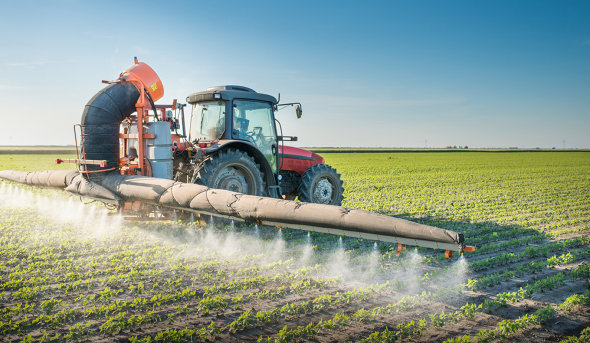
\includegraphics[width=9.5cm]{pestizide}
	\caption{Pestizide werden auf dem Feld verteilt.}
\end{wrapfigure}
In einer umfassenden Studie\\\cite{_reportweintesting-1.pdf} wurde von Greenpeace Schweiz sechs
Weinberge in verschiedenen Weinbauregionen auf Pestizide untersucht. Insgesamt wurden 33 Wirkstoffe
festgestellt von denen 23 auf der Greenpeace "Blacklist" stehen. Dies bedeutet diese Wirkstoffe sind
entweder humantoxisch oder haben eine inakzeptable Wirkung auf das Ökosystem. Zwei der gefunden
Wirkstoffe waren sogar durch die EU nicht zugelassen. In den Böden konnten ältere Pestizide
nachgewiesen werden, welches aufzeigt,  dass sich manche Pestizide nur sehr langsam abbauen und über
Jahrzehnte Schäden in den Ökosystemen anrichten. In der Studie wurden auch die fertigen Weine auf
ihre Inhalte überprüft. In der konventionellen Weinprodukten wurden vermehrt Rückstände von
Pestiziden gefunden, welche aber die Grenzwerte nicht überschritten. Allerdings gibt es für Weine auch nur selten Pestizid Grenzwerte. Wie in Abbildung \ref{fig:ha} dargestellt, ist die UBP von ÖLN ein wesentlicher Bestandteil der gesamten Belastung. Der Unterschied zur biologischen Produktion wird deutlich, die eine Anwendung von Pestiziden verbietet.
 \begin{figure}[H]	
	\centering
	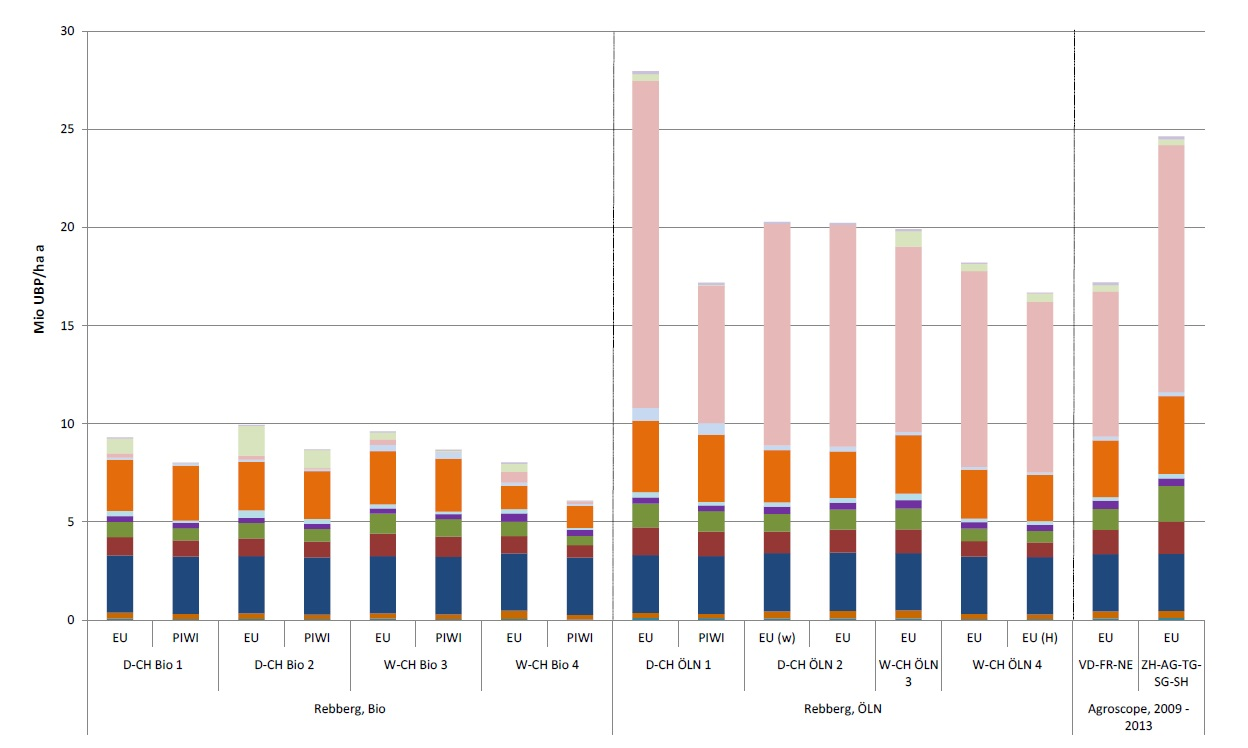
\includegraphics[width=0.9\textwidth]{auswirkungen}
	\caption{Gesamtumweltbelastung [UBP] der ÖLN- und biologischen Bewirtschaftung einer Hektare Rebbergs}
	\label{fig:ha}
\end{figure}

\subsubsection{Kalifornien}
\label{sub:sch_dlingsbek_mpfung}

Das Ziel der Schädlingsbekämpfung in Kalifornien ist nicht das komplette Ausrotten oder Verhindern
der Schädlinge. Es werden stattdessen Schwellenwerte definiert. Es werden erst Massnahmen getroffen,
wenn diese Schwellenwerte erreicht oder überschritten werden. Diese Massnahmen umfassen biologische,
kulturelle und chemische Mittel, die so eingesetzt werden, dass ökonomische, Umwelt- und
Gesundheitsrisiken minimiert werden.

Um den Einsatz von giftigen Pestiziden zu verringern, werden diese erst eingesetzt, wenn es wirklich
nötig ist. Das setzt eine kontinuierliche Kontrolle über den Schädlingsbefall voraus. Dies wird von
etwa drei Viertel der Weinbauern vorgenommen.

Als Prävention werden kulturelle Massnahmen getroffen. Dazu gehören das Entfernen von Laub, Hecken,
Staubkontrolle und Bewässerung.

\cite{_2015_cswa_sustainability_report.pdf}\\
\cite{_2015_report_appendix.pdf}


Zu den biologischen Schädlingsbekämpfungsmittel gehören natürliche Feinde wie Spinnen, Marienkäfer
oder Wespen, aber auch Hühner oder Schafe, die gegen Erdraupen oder zum Mähen von Gräsern eingesetzt
werden \cite{_sustainable}.  Durch diese Massnahmen werden weniger
Pestizide eingesetzt und die Artenvielfalt wird erhöht.
